%% Compile with       pdflatex --jobname=demo-prot1-fig demo-prot1.tex

\documentclass{article}

\usepackage{amsmath}
\usepackage{amstext}
\usepackage{amssymb}
\usepackage{amsfonts}
\usepackage{xspace}
\usepackage{graphicx}
\usepackage{url}
\usepackage{mdwlist}
\usepackage{courier}
\usepackage{lscape}
\usepackage{comment}
\usepackage{wrapfig}
\usepackage{multirow}
\usepackage{bussproofs}
\usepackage{pdftricks}
\usepackage{cite}
\usepackage{footmisc}
\usepackage{balance}
\usepackage{enumerate}
\usepackage[normalem]{ulem}
\usepackage{hyperref}
\usepackage{tikz}
\usetikzlibrary{calc,backgrounds,automata,arrows}
\pgfrealjobname{demo-prot1-cex-5}

\begin{document}

\beginpgfgraphicnamed{demo-prot1-cex-5-fig}
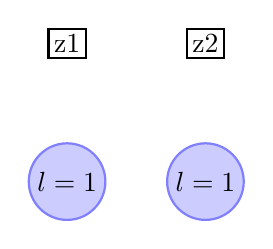
\begin{tikzpicture}
 \tikzstyle{arrow} = [->,shorten >=1pt,>=stealth'];
 \tikzstyle{place3} = [circle,thick,node distance=5em,inner sep=0.2em];
 \tikzstyle{placez1} = [thick,node distance=5em,inner sep=0.2em];
 \tikzstyle{placez2} = [thick,node distance=5em,inner sep=0.2em];
 \tikzstyle{placeZ1} = [draw=black,fill=white];
 \tikzstyle{placeZ2} = [draw=black,fill=white];
 \tikzstyle{placeY} = [draw=black,fill=white];
 \tikzstyle{placeB} = [draw=blue!50,fill=blue!20];
 \tikzstyle{placeR} = [draw=red!50,fill=red!20];
 \tikzstyle{placeG} = [draw=green!50,fill=green!20];
 \tikzstyle{placeW} = [draw=black!50,fill=black!10];

 \node[placez1,placeZ1,name=z1] {z1};  
 \node[placez2,placeZ2,name=z2, right of=z1] {z2};
 \node[place3,placeB, below of=z1]   {$l=1$}; 
 \node[place3,placeB, below of=z2]   {$l=1$};

\end{tikzpicture}
\endpgfgraphicnamed

\end{document}


